
%%%%%%%%%%%%%%%%%%%%%%%%%%%%%%%%%%%%%%%%%%%%%%%%%%%%%%%%%%%%%%%%%%%%%
%% This is a (brief) model paper using the achemso class
%% The document class accepts keyval options, which should include
%% the target journal and optionally the manuscript type.
%%%%%%%%%%%%%%%%%%%%%%%%%%%%%%%%%%%%%%%%%%%%%%%%%%%%%%%%%%%%%%%%%%%%%
\documentclass[journal=apchd5,manuscript=article]{achemso}

%%%%%%%%%%%%%%%%%%%%%%%%%%%%%%%%%%%%%%%%%%%%%%%%%%%%%%%%%%%%%%%%%%%%%
%% Place any additional packages needed here.  Only include packages
%% which are essential, to avoid problems later. Do NOT use any
%% packages which require e-TeX (for example etoolbox): the e-TeX
%% extensions are not currently available on the ACS conversion
%% servers.
%%%%%%%%%%%%%%%%%%%%%%%%%%%%%%%%%%%%%%%%%%%%%%%%%%%%%%%%%%%%%%%%%%%%%
\usepackage[version=3]{mhchem} % Formula subscripts using \ce{}
\usepackage[T1]{fontenc}       % Use modern font encodings
\usepackage{graphicx}
\usepackage{amsmath}
\usepackage{xcolor}
\usepackage{wrapfig}
%%%%%%%%%%%%%%%%%%%%%%%%%%%%%%%%%%%%%%%%%%%%%%%%%%%%%%%%%%%%%%%%%%%%%
%% If issues arise when submitting your manuscript, you may want to
%% un-comment the next line.  This provides information on the
%% version of every file you have used.
%%%%%%%%%%%%%%%%%%%%%%%%%%%%%%%%%%%%%%%%%%%%%%%%%%%%%%%%%%%%%%%%%%%%%
%%\listfiles

%%%%%%%%%%%%%%%%%%%%%%%%%%%%%%%%%%%%%%%%%%%%%%%%%%%%%%%%%%%%%%%%%%%%%
%% Place any additional macros here.  Please use \newcommand* where
%% possible, and avoid layout-changing macros (which are not used
%% when typesetting).
%%%%%%%%%%%%%%%%%%%%%%%%%%%%%%%%%%%%%%%%%%%%%%%%%%%%%%%%%%%%%%%%%%%%%
\newcommand*\mycommand[1]{\texttt{\emph{#1}}}

%%%%%%%%%%%%%%%%%%%%%%%%%%%%%%%%%%%%%%%%%%%%%%%%%%%%%%%%%%%%%%%%%%%%%
%% Meta-data block
%% ---------------
%% Each author should be given as a separate \author command.
%%
%% Corresponding authors should have an e-mail given after the author
%% name as an \email command. Phone and fax numbers can be given
%% using \phone and \fax, respectively; this information is optional.
%%
%% The affiliation of authors is given after the authors; each
%% \affiliation command applies to all preceding authors not already
%% assigned an affiliation.
%%
%% The affiliation takes an option argument for the short name.  This
%% will typically be something like "University of Somewhere".
%%
%% The \altaffiliation macro should be used for new address, etc.
%% On the other hand, \alsoaffiliation is used on a per author basis
%% when authors are associated with multiple institutions.
%%%%%%%%%%%%%%%%%%%%%%%%%%%%%%%%%%%%%%%%%%%%%%%%%%%%%%%%%%%%%%%%%%%%%
\author{Nicholas P. Montoni}
\author{Steven C. Quillin}
\author{Charles Cherqui}
\author{David J. Maisello}
\affiliation[Department of Chemistry, University of Washington]
{Department of Chemistry, University of Washington, Seattle, WA 98195}
\email{masiello@chem.washington.edu}

%%%%%%%%%%%%%%%%%%%%%%%%%%%%%%%%%%%%%%%%%%%%%%%%%%%%%%%%%%%%%%%%%%%%%
%% The document title should be given as usual. Some journals require
%% a running title from the author: this should be supplied as an
%% optional argument to \title.
%%%%%%%%%%%%%%%%%%%%%%%%%%%%%%%%%%%%%%%%%%%%%%%%%%%%%%%%%%%%%%%%%%%%%
\title[]
    {Quantifying the Role of Retardation Effects in Magnetic Plasmon Supporting Metal Nanoparticle Arrays}
%%%%%%%%%%%%%%%%%%%%%%%%%%%%%%%%%%%%%%%%%%%%%%%%%%%%%%%%%%%%%%%%%%%%%
%% Some journals require a list of abbreviations or keywords to be
%% supplied. These should be set up here, and will be printed after
%% the title and author information, if needed.
%%%%%%%%%%%%%%%%%%%%%%%%%%%%%%%%%%%%%%%%%%%%%%%%%%%%%%%%%%%%%%%%%%%%%
\abbreviations{MNP, LSPR, EELS}
\keywords{plasmon, hybridization, magnetic, retardation}

%%%%%%%%%%%%%%%%%%%%%%%%%%%%%%%%%%%%%%%%%%%%%%%%%%%%%%%%%%%%%%%%%%%%%
%% The manuscript does not need to include \maketitle, which is
%% executed automatically.
%%%%%%%%%%%%%%%%%%%%%%%%%%%%%%%%%%%%%%%%%%%%%%%%%%%%%%%%%%%%%%%%%%%%%
\begin{document}

%%%%%%%%%%%%%%%%%%%%%%%%%%%%%%%%%%%%%%%%%%%%%%%%%%%%%%%%%%%%%%%%%%%%%
%% The "tocentry" environment can be used to create an entry for the
%% graphical table of contents. It is given here as some journals
%% require that it is printed as part of the abstract page. It will
%% be automatically moved as appropriate.
%%%%%%%%%%%%%%%%%%%%%%%%%%%%%%%%%%%%%%%%%%%%%%%%%%%%%%%%%%%%%%%%%%%%%
\begin{tocentry}

Some journals require a graphical entry for the Table of Contents.
This should be laid out ``print ready'' so that the sizing of the
text is correct.

Inside the \texttt{tocentry} environment, the font used is Helvetica
8\,pt, as required by \emph{Journal of the American Chemical
Society}.

The surrounding frame is 9\,cm by 3.5\,cm, which is the maximum
permitted for  \emph{Journal of the American Chemical Society}
graphical table of content entries. The box will not resize if the
content is too big: instead it will overflow the edge of the box.

This box and the associated title will always be printed on a
separate page at the end of the document.

\end{tocentry}

%%%%%%%%%%%%%%%%%%%%%%%%%%%%%%%%%%%%%%%%%%%%%%%%%%%%%%%%%%%%%%%%%%%%%
%% The abstract environment will automatically gobble the contents
%% if an abstract is not used by the target journal.
%%%%%%%%%%%%%%%%%%%%%%%%%%%%%%%%%%%%%%%%%%%%%%%%%%%%%%%%%%%%%%%%%%%%%
\begin{abstract}
Magnetic plasmons, the collective response of cyclic arrangements of electric plasmon-supporting metal nanoparticles, have been of recent theoretical and experimental interest. As magnetic-plasmon-supporting aggregates are often large (hundreds of nanometers to microns in size), information takes time to propagate across such nanostructures. As a result, they are not well-described in the quasistatic limit with plasmon hybridization theory. In this Letter it is shown that for small magnetic oligomers the quasistatic approximation is sufficient, but, as the systems grow in size, retardation effects must be considered. The quasistatic tight-binding model can be manipulated to include retardation effects by utilizing the full electric field of a dipole. This fully retarded tight-binding model accurately predicts the energy-ordering of magnetic plasmon modes in agreement with full-wave simulations.
\end{abstract}

%%%%%%%%%%%%%%%%%%%%%%%%%%%%%%%%%%%%%%%%%%%%%%%%%%%%%%%%%%%%%%%%%%%%%
%% Start the main part of the manuscript here.
%%%%%%%%%%%%%%%%%%%%%%%%%%%%%%%%%%%%%%%%%%%%%%%%%%%%%%%%%%%%%%%%%%%%%
When two or more metal nanoparticles (MNPs) are brought together, their individual electric plasmons can hybridize to produce new, collective plasmon resonances\cite{Lucas1976,ARAVIND1981,Xu1995,Mischenko1995}. Arranging three or more MNPs on the vertices of a polygon generates a collective mode that resembles a fictitious current loop and produces a sizeable magetic moment in the center of the polygon\cite{Alu2006,Alu2008,Liu2011,Nord2006,Cherqui2014}. These aggregates can couple to and enhance the magnetic field of light, leading to applications such as solar cell enhancement\cite{Graydon2011,Alu2014solar,Le2015solar}, biosensing and detection\cite{Zia2010trans,Noginova2008trans,Wang:13,Fan2015,Wei2015,Shvets2012,Altug2012bio,Nord2011fano}, and information storage and propagation\cite{Zhang2006,NordHal2011,NordHal2012}.

Of recent interest has been the ability of magnetic plasmons, much like electric plasmons, to hybridize\cite{Cherqui2016}. Similar to how a pair of electric plasmons can produce an electrically bright and an electrically dark mode, a pair of magnetic plasmons can produce a magnetically bright mode and a magnetically dark mode. This understanding opens up new routes to preferentially exciting magnetic and electric plasmons and distinguishing between the different plasmonic modes of a particular aggregate. Studies of the properties of magnetic plasmons have focused on plasmon propagation and hybridization, but have not sought to determine under what circumstances the magnetic plasmons of a system dominate its optical properties. Key to answering this question is the influence of retardation effects.

Much work has been done on magnetic plasmons in the quasistatic limit, which assumes that electromagnetic information propagates infinitely quickly. While retardation effects have been considered in studies of both large MNPs and infinite MNP arrays\cite{Abajo2008,Gu2010,vonPlessen2007,Rechbacher2003,Kottman2001,Schatz2003,Royer2005,Chumanov2010}, they have never been incorporated into models of intermediate-sized MNP arrays. Certainly, the single particle, single oligomer, and infinite system limits have been well-studied while the size regime in between is still relatively uncharted[\textbf{Kagan2017}]. This paper will show that, contrary to intuition, retardation effects play a significant role in the optical properties of magnetic-plasmon-supporting MNP aggregates int he intermediate size regime. It will be shown that by incorporating retardation effects into a simple model, the magnetic mode frequencies can be accurately predicted. Following this, it will be shown that the spectral order of the magnetic modes can be directly controlled, and that due to the specific radiative properties of each magnetic mode, it is possible to track one of the magnetic modes as a function of energy, scale, and size. Finally, the magnetic and electric plasmons on single oligomers will be shown to interfere in such a way as to produce unidirectional radiation. The tracking of the magnetic modes and their interference with the electric modes is the key to determining when retardation effects must be included to produce an accurate model.

This work utilizes and augments a previously published tight-binding model\cite{Cherqui2014}. The model in question maps the electric plasmon of each nanoparticle onto a harmonic oscillator and allows them to couple through quasistatic, near-field interactions using the Hamiltonian

\begin{equation}
\frac{H}{\hbar\omega_{\textrm{sp}}} = \frac{1}{2}\sum_{i}\left[\boldsymbol{\Pi}_{i}^2 + \textbf{Q}_{i}^{2}\right] - \frac{\alpha_{\textrm{sp}}}{2}\sum_{i\neq j}\textbf{Q}_{i}\cdot\boldsymbol{\Lambda}_{ij}\cdot\textbf{Q}_{j}.
\label{full_hammy}
\end{equation}

Here, $\omega_{\textrm{sp}}$ is the resonant frequency of the individual electric plasmons, the $\boldsymbol{\Pi}_{i}$ are the generalized momenta conjugate to the generalized coordinates $\textbf{Q}_{i}$, $\alpha_{\textrm{sp}}$ is the polarizability of each individual MNP, and $\boldsymbol{\Lambda}_{ij}$ is the near-field dipole-dipole relay tensor. In this work, retardation effects are incorporated into the dipole-dipole relay tensor through the intermediate- and far-field terms in the dipole electric field as follows:

\begin{equation}
\boldsymbol{\Lambda}_{ij} = \left[\left(\frac{1}{r_{ij}^3} - \frac{\textrm{i}\omega}{cr_{ij}^2}\right)\left(3\hat{\textbf{n}}_{ij}\hat{\textbf{n}}_{ij} - \textbf{1}\right) + \frac{\omega^2}{c^2r_{ij}}\left(\textbf{1} - \hat{\textbf{n}}_{ij}\hat{\textbf{n}}_{ij}\right)\right]e^{\textrm{i}\omega/c r},
\label{dipoledipole}
\end{equation}

where $r_{ij}$ is the distance between the $i^{\textrm{th}}$ and $j^{\textrm{th}}$ dipoles along the unit vector $\hat{\textbf{n}}_{ij}$, \textbf{1} is the unit dyad, $c$ is the speed of light, and $\omega$ is the collective frequency at which all of the dipoles oscillate. Using Equations~\ref{full_hammy} and ~\ref{dipoledipole}, Hamilton's equations of motion,

\begin{equation}
\ddot{\textbf{Q}}_{i} = -\textbf{Q}_{i} + \sum_{j\neq i}\boldsymbol{Lambda}_{ij}\cdot\textbf{Q}_{j}
\label{eom}
\end{equation}

 can be found and the system of equations can be solved for the eigenvalues and eigenvectors of the nanoparticle array. The eigenvectors are the generalized coordinates corresponding to each dipole moment in the aggregate. It is important to note that because the eigenvalues, the collective frequencies, appear in the coupling terms, this will result in a system of transcendental equations which must be solved iteratively. 

In this paper, three model systems are considered. Following previous work, the model systems are constructed from fused, six-member rings of silver nanospheres, resembling conjugated hydrocarbon rings. The aggregates considered are a two-ring system, a linear three-ring system, and a triangular three-ring system. Solving for the magnetic eigenmodes of each system results in a set of eigenvectors for each mode which correspond to electric dipole moments. Figure~\ref{field_plots} shows the oligomers, the dipole moments on each sphere, and the magnetic field distribution computed from\cite{jackson_classical_1999}

\begin{equation}
\textbf{B}_{\textrm{tot}}(\textbf{r},\omega) = \frac{\omega^2}{c^2}\sum_{j}(\hat{\textbf{n}}_{j}\times\textbf{p}_{j})\frac{e^{\textrm{i}\omega/c r_j}}{r_j}\left(1 - \frac{c}{\textrm{i}\omega r_{j}}\right).
\label{magnetic_field}
\end{equation}

\begin{figure}
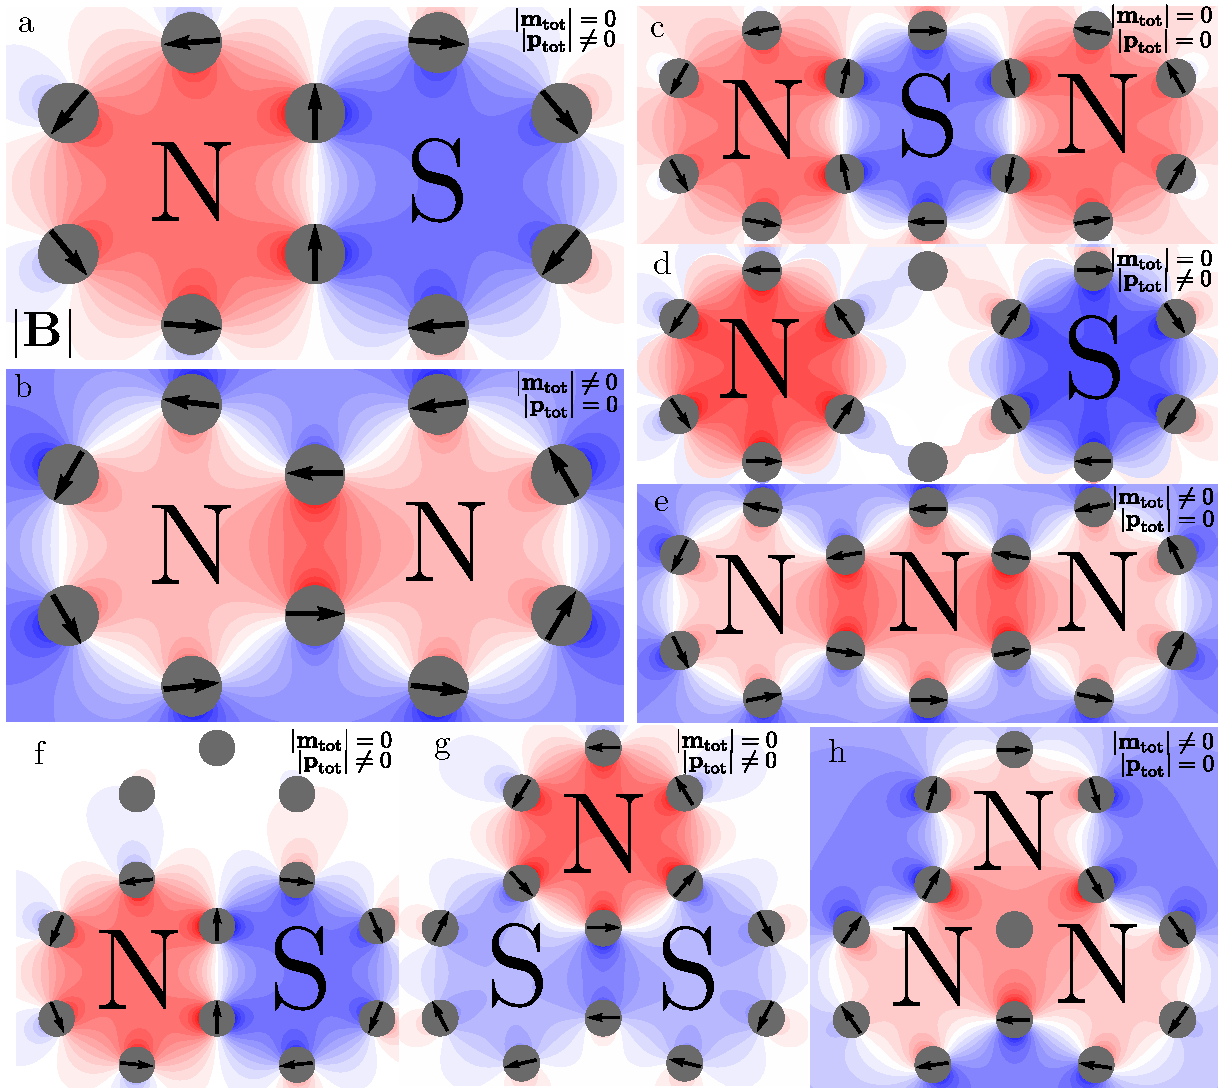
\includegraphics[width=7in]{fields_new_arrows.pdf}
\caption{Magnetic fields produced by each of the magnetic eigenmodes of the twomer (a and b), 1D threemer (c, d, and e), and 2D threemer (f, g, and h). The magnetic field distributions and orientation of electric dipoles can be used to determine whether each magnetic mode is magnetically or electrically bright of dark. Red regions are labeled ``N'' for ``North'' and ``S'' for ``South'' in reference to the north and south poles of a magnet. As such, the modes are referred to by their associated aggregate and acronym.}
\label{field_plots}
\end{figure}

From the magnetic field distributions and the orientation of electric dipoles, some key observations can be made about the magnetic modes. The in-phase magnetic mode of each oligomer (Figure~\ref{field_plots}b, e, and h) has a net magnetic dipole, meaning it will couple to the magnetic field of light. The out-of-phase magnetic modes in Figure~\ref{field_plots}a, d, f, and g all have net electric dipole moments, so they will interact with the electric field of light. The magnetic mode in Figure~\ref{field_plots} has no dipole moments at all, making it optically dark. The classification of electrically bright and magnetically bright will play an important role in later discussion.

With the model producing the correct eigenmodes, it can now be used to show how properties such as scale of the oligomer and separation distance between MNPs impact the eigenvalues. To do this, a nearest neighbor distance is defined as $r_{nn} = (s+2)a_0$ where $a_0$ is the particle radius and $s$ is a face-to-face distance in units of $a_0$. Figure~\ref{scaling}a shows the magnetic eigenmode frequencies as a function of oligomer scale. This is calculated by fixing the parameter $s=1$ and varying $a_0$ from 1 nm to 30 nm. It can be seen for all three oligomers that at $a0 = 5$ nm the in-phase magnetic mode becomes the lowest in energy, contrary to predictions made by models in past work. Even more interesting is that the eigenmodes change spectral order again at 25 nm. Figure~\ref{scaling}a also includes comparison to simulation, showing that the model overestimates the eigenvalues by about 0.05 eV. 

\begin{figure}
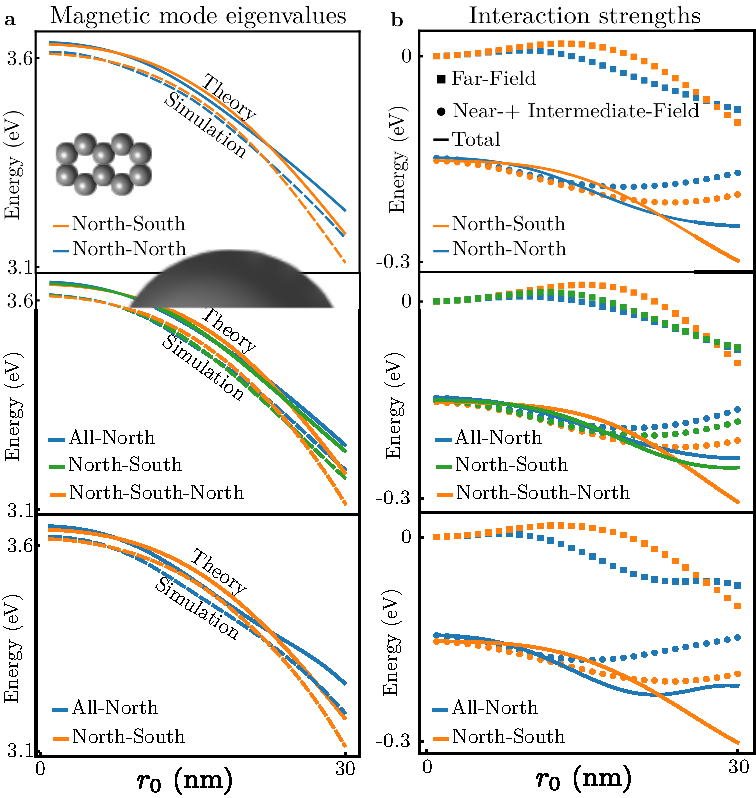
\includegraphics[width=7in]{scale_eigs.pdf}
\caption{Theoretical and simulated magnetic mdoe eigenvalues (a) and total, near plus intermediate, and far interaction strengths (b) plotted as a function of system scale. Each row corresponds to one of the oligomer systems studied in this work. In column (a), note that the eigenvalues all decrease with increasing $r_0$, but the eigenvalues cross at 5 nm and 21 nm. This is corroborated by full-wave simulation (dashed lines). Interestingly, these crossings are mirrored in (b) by the fluctuations in the far-field (squares) interaction. By themselves, the near- and intermediate-fields (circles) would never contribute any mode crossings to the total interaction (solid). Due to the opposite inflection of the far-field interaction, however, the crossings become possible.}
\label{scaling}
\end{figure}

Spectral switching of eigenmodes is counterintuitive and unexplored. In order to more fully explain why this could happen, Figure~\ref{scaling}b shows the total interaction strengths between dipoles in each eigenmode. More specifically, the total strength is computed, as well as the sum of the near- and intermediate-field strengths, followed by the far-field strength separately. This breakdown shows that the eigenmode crossings are due entirely to the far-field interaction. There are no crossings exhibited in the near- and intermediate-field terms, so these contribute only to net shifting of the eigenmodes. It is the change in relative magnitude of the far-field interaction that causes the eigenmodes to change spectral order. This is the most important point to take away from these plots: the far-field term is the magnetic term, and so it alone gives a measure of the importance of magnetic effects on these systems. And from these plots, it would seem that it becomes important for particles as small as 5 nm, and for separation distances between 15 nm and 50 nm.

Aggregate scale is not something that can be easily manipulated in real time in a laboratory, as it would require the refrabrication of a different aggregate for each experiment. However, recent research has focused on the ability of DNA and polymers to change shape and size in response to stimuli such as heat and pH[\textbf{cite Odom, Ginger, Schatz}]. Specifically, these techniques have been used to continuously and reversibly tune the aggregation scheme of a MNP array. Using this concept, the following set of calculations varies the nearest neighbor spacing, $r_{nn}$ by varying $s$ from 0 to 10 and keeping $a_0$ constant at 15 and 30 nm.

\begin{figure}
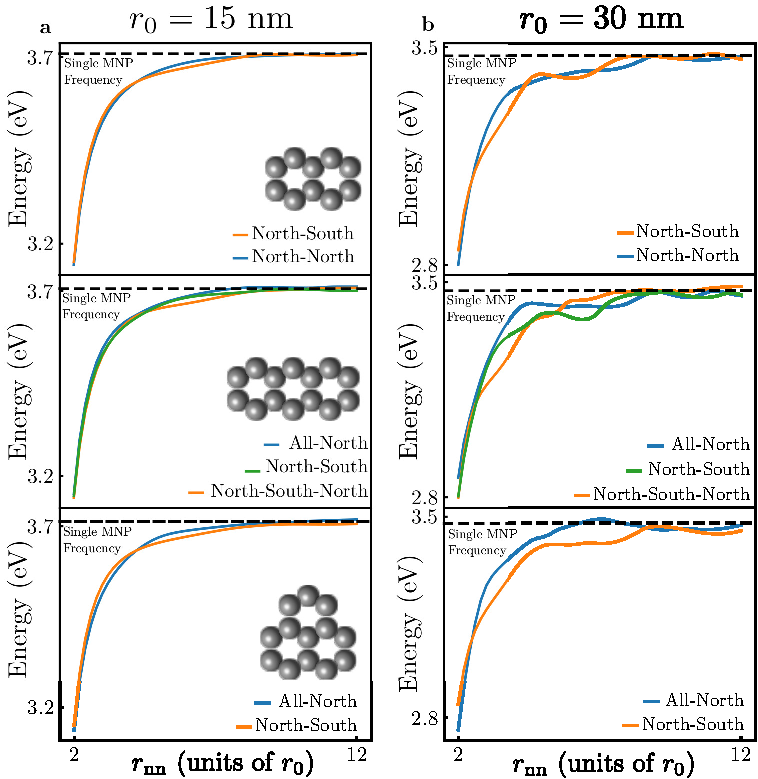
\includegraphics[width=7in]{spacing_study.pdf}
\caption{}
\label{spacing}
\end{figure}

Figure~\ref{spacing}a shows the eigenvalues of each oligomer as a function of spacing for the 15 nm radius particles. As the space between particles increases, the magnetic modes collectively increase in energy, tending towards the single plasmon resonant frequency. The eigenvalues appear to cross and exhibit slight oscillatory motion. The crossings and oscillations are much more pronounced for the 30 nm particles (Figure~\ref{spacing}b). This is interesting because it shows that magnetic oligomers show a high degreee of spectral tunability. It can be seen that the energy order of the magnetic modes depends on a parameter that can be manipulated in a laboratory. This versatility could be exploited to design optical magnetic switches and detectors.

There is a drawback in this line of reasoning, however. The splitting between the magnetic modes is very small, on the order of hundredths of electron volts, tenths at the most. In order to fully utilize magnetic oligomers, a technique is required to unravel these overlapping modes. Because the magnetic modes exhibit distinct, orthogonal magnetic and electric dipole moments, they can be individually or mutually excited by incoming light. Furthermore, because the dipole moments have orthogonal orientations, they scatter light in different directions. Finally, when the modes are mutually excited, they can interfere with each other to produce unidirectional radiation[\textbf{cite Kivshar and others}]. These properties are explored both as a way to observe the magnetic modes and as a way to quantify the importance of retardation effects. Because there are techniques that can measure the angular distribution of scattered light from a nanomaterial, this is presented as a way to infer the importance of the in-phase magnetic mode[\textbf{cite two papers measuring angular scattering}].

In planar plasmonic oligomers, the magnetic and electric collective plasmons are orthogonal to each other (see Figure~\ref{field_plots}. Because of this, it is possible to probe multiple modes with a single laser polarization, specifically one in which the magnetic field of the incident light is directed through the rings of the oligomer. Because of the breadth and overlap of the magnetic modes, this will make it possible to observe both at once, but more importantly, this will make it possible to detect the point at which the magnetic plasmons dominate the spectrum.

The angular distribution of power scattered by the olgiomers from the light polarization descibed above is dependent on the size of the oligomer and the frequency at which the light is collected. Here, the angular distribution is calculated from

\begin{equation}
\frac{dP}{d\Omega} = \frac{c}{8\pi}\textrm{Re}[r^2 \hat{\textbf{n}}\cdot \sum_i \textbf{E}_i \times \sum_j \textbf{B}_j]\\
= \frac{\omega^4}{8\pi c^3}\textrm{Re}[\hat{\textbf{n}}\cdot \left(\sum_i \left(\frac{\textbf{r}-\textbf{r}_i}{r}\times\textbf{p}_i\right)\times\frac{\textbf{r}-\textbf{r}_i}{r}\right)\textrm{e}^{\textrm{i}k|\textbf{r}-\textbf{r}_i|} \times \sum_j\left(\frac{\textbf{r}-\textbf{r}_j}{r}\times\textbf{p}_j\right)\textrm{e}^{\textrm{i}k|\textbf{r}-\textbf{r}_i|}
\label{diff_power_full}
\end{equation}

where at every point $\textbf{r}$ on the flux screen the fields scattered by each dipole located at positions $\textbf{r}_i$ are added together before the cross product is taken. There are two relevant limits to take: one in which the loop of dipoles is very small ($\textbf{r}_i = \textbf{0}$) and one in which the loop is finite in size, but the detector is infinitely far away ($r = \infty$). Taking the first limit results in

\begin{equation}
\frac{dP}{d\Omega} = \frac{\omega}{8\pi c r^2}|\textbf{m}|^2
\label{mag_dp}
\end{equation}

a term which decays to zero for a flux screen at infinity. Allowing the loop to have finite size, however, introduces phase effects. It is these that contribute to the overall radiation of the loops of dipoles. Keeping the exponential terms and again letting the magnetic dipole terms decay to zero gives

\begin{equation}
\frac{dP}{d\Omega} = \frac{ck^4}{8\pi}\sum_{ij}[\textbf{p}_i\textbf{p}_j - (\textbf{p}_i\cdot\hat{\textbf{n}})(\textbf{p}_j\cdot\hat{\textbf{n}})]\textrm{e}^{\textrm{i}k\hat{\textbf{n}}\cdot(\textbf{r}_j-\textbf{r}_i)}.
\label{dipoles_only_dp}
\end{equation}

From this, it can be seen that the radiation pattern of a collection of dipoles, regardless of arrangement, is dependent only on the orientations and locations of the dipoles in relation to one another. This equation can be used to gain insight into the angular dependence of the scattered light of collections of dipoles and to exlpain the results from numerical simulations. The results of those simulations are shown and discussed below.

\begin{figure}
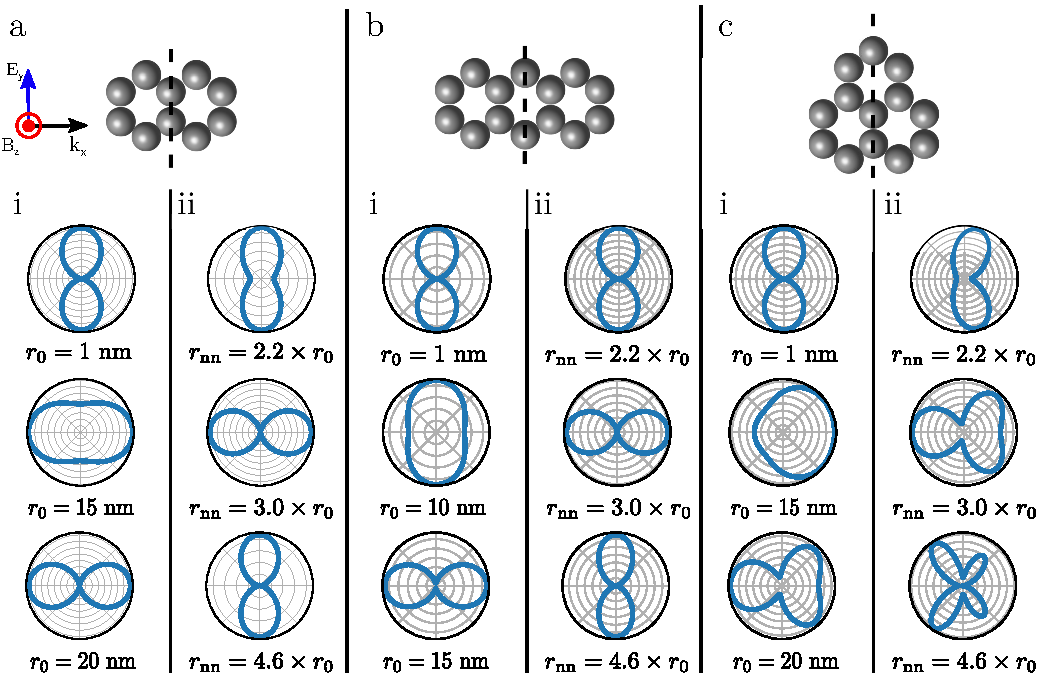
\includegraphics[width=5in]{polar_plots_yz.pdf}
\label{polar_plots_yz}
\end{figure}

Figure~\ref{polar_plots_yz} shows this analysis in depth. The radiation pattern collected at the in-phase magnetic plasmon frequency of the twomer system is plotted in the plane containing the electric and magnetic field as a function of both scale and spacing. At small scalings, the scattered power appears to be entirely due to the electric plasmons. As the systems get larger, the magnetic scattered radiation dominates the pattern. This can be further seen in the scaling calculations, where the radiation pattern at a specific frequency changes from electric-dominated to magnetic-dominated and back again. This is significant because it is the first step towards identifying and observing the phenomenon of magnetic mode switching. By watching a particular frequency and varying some system parameter, the radiation pattern can be shown to change. These results are even more significant because they show that even with particles as small as 10 nm in radius, retardation effects have a measureable impact on the optical properties of MNP aggregates.

\begin{figure}
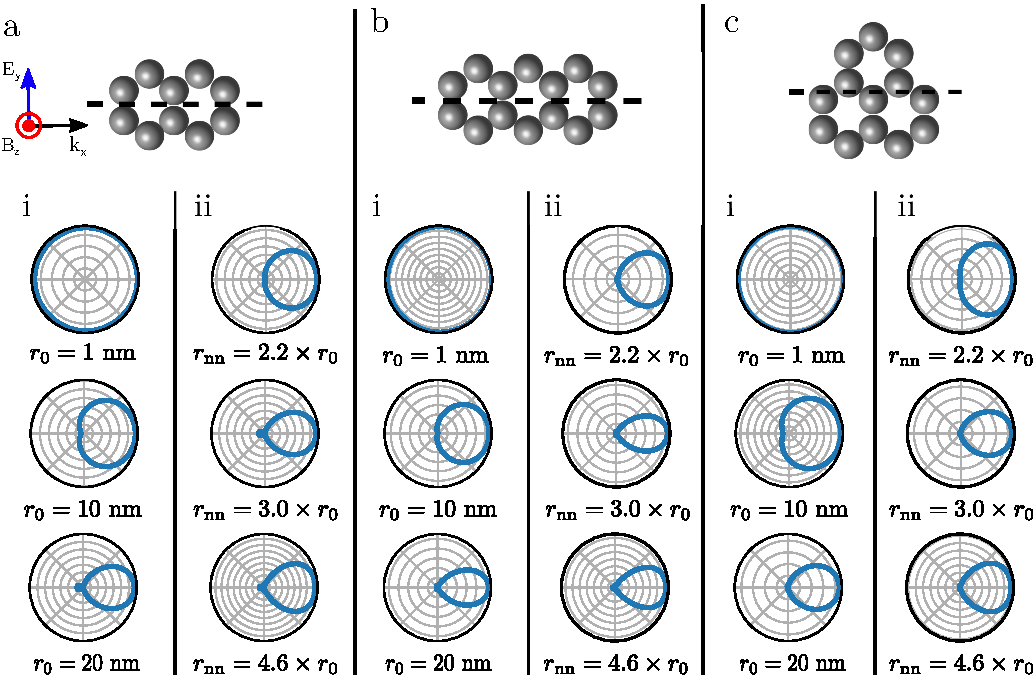
\includegraphics[width=5in]{beaming.pdf}
\label{polar_plots_xz}
\end{figure}

Changing the plane in which radiation is collected from these systems reveals another interesting property of magnetic plasmon oligomers. Collecting scattered light in the plane perpendicular to the previous set of calculations gives another measure of the role of retardation effects. When the magnetic and electric plasmons are of commensurate strength, their fields interfere destructively in some regions of space and constructively in others, leading to directionality in their emitted light. This can be seen in Figure~\ref{polar_plots_xz}. As a function of scale, the radiation pattern can be seen to shift from pure electric dipole to unidirectional, and at large scalings, more magnetic in character. Similarly, as a function of spacing it can be seen that the unidirectionality dominates at certain energies and configurations. However, unlike the distinctive radiation patterns from the previous section, it would seem that once the magnetic plasmons are strong enough to interfere with the electric plasmons, the interference effects never truly go away, except in the case of particles infinitely far away from each other. According to equation [\textbf{PUT IN THAT EQUATION WHEN YOU'RE DONE AND SURE}], there is a sweet spot where the magnetic and electric plasmons can maximally interefere, and it occurs when they of nearly equal magnitude. This result is significant because it is the most convincing evidence yet that magnetic effects matter and contribute significantly to the optical properties of MNP aggregates. The point where the magnetic and electric plasmons maximally interfere is the point where magnetic, and by extension, retardation effects, matter most.

Even more interestingly, this phenomenon appears to break down with increasing length of the oligomer chain. Looking at chains of three, four, five, ten, and twenty oligomers, the beaming capabilities decrease as the chains become longer. This is further evidence of the idea the magnetic and electric dipole modes must be of commensurate strength in order to interfere and produce unidirectional radiation. Chains of magnetic oligomers behave much like particle-in-a-box states; this can be seen in the nodal structure of the twomer and linear threemer in Figure~\ref{field_plots}. As the chains become longer, the magnetic modes will exhibit increasingly dilute field density, leading to weak interferences between modes. As a result, the radiation emitted by these structures loses its directionality. This is important because it emphasizes the significance of smaller magnetic oligomers as the perfect tools to understanding magnetic plasmons and retardation effects. The lack of unidirectionality of longer chains is displayed in Figure ~\ref{bad_beaming}.

Magnetic plasmon supporting aggregates consisting of few oligomers are excellent tools for analyzing the role of retardation effects on MNP aggregates. More conclusion.

\section{Future Work}

\begin{acknowledgement}
CEI, Niket, Harrison, HPC/Hyak/Mox.
\end{acknowledgement}

%%%%%%%%%%%%%%%%%%%%%%%%%%%%%%%%%%%%%%%%%%%%%%%%%%%%%%%%%%%%%%%%%%%%%
%% The appropriate \bibliography command should be placed here.
%% Notice that the class file automatically sets \bibliographystyle
%% and also names the section correctly.
%%%%%%%%%%%%%%%%%%%%%%%%%%%%%%%%%%%%%%%%%%%%%%%%%%%%%%%%%%%%%%%%%%%%%
\bibliography{references}
\end{document}
